\documentclass{article}
\usepackage{graphicx}


\begin{document}

Liouville’s Theorem states that the flow of a Hamiltonian system preserves phase space volume. In the context of statistical mechanics this means that the phase space volume is conserved as microstates evolve in line with our hamiltonian equations of motion. From the fundamental postulate of statistical mechanics we know that the entropy of the macrostate depends on the volume of the phase space by the formula $S = K_{B} ln |\Gamma| $. Therefore, if phase space volume changes, so does the entropy. If it were not for Liouville’s theorem then, the movement of particles in phase space for a given macrostate could cause a change in phase space volume that would affect the extensive variables of the system’s macrostate. At equilibrium, a system should not change in extensive properties like entropy or temperature without external changes that affect the internal energy of the system, so Liouville’s theorem allows us to use equilibrium statistical mechanics. Transformations in phase space that conserve phase space volume are illustrated in the figure below:

\begin{centering}

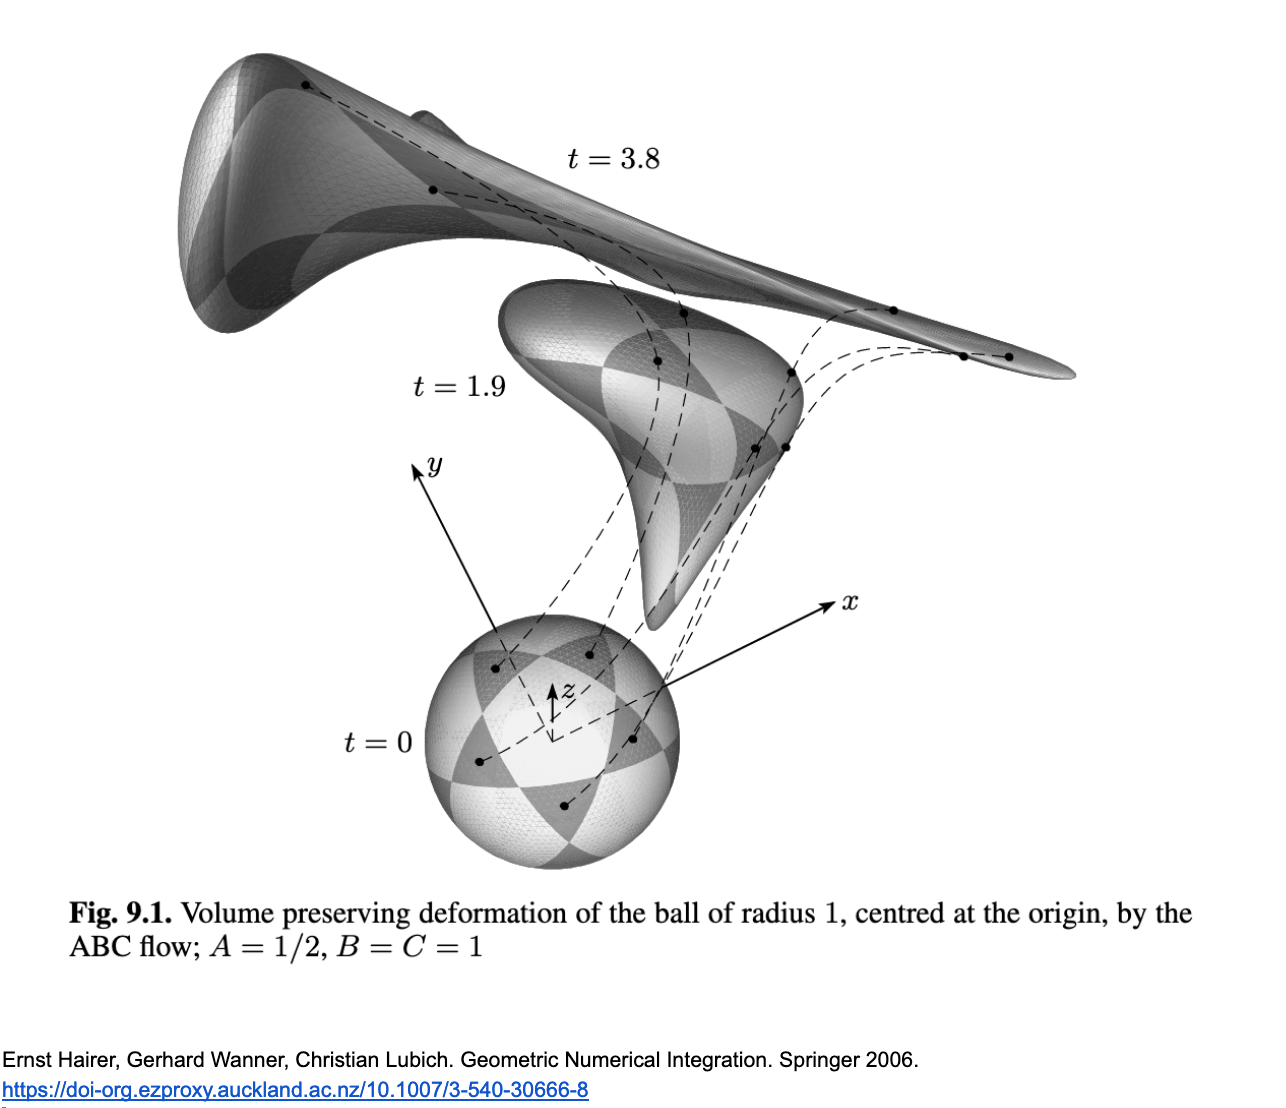
\includegraphics[scale=0.4]{aferLiouvillefigure.png}

\end{centering}







\end{document}